\hypertarget{a00005}{
\section{Dokumentacja klasy parser}
\label{dd/dad/a00005}\index{parser@{parser}}
}
{\tt \#include $<$parser.hpp$>$}

Diagram współpracy dla parser:\nopagebreak
\begin{figure}[H]
\begin{center}
\leavevmode
\includegraphics[width=189pt]{d9/d73/a00060}
\end{center}
\end{figure}
\subsection*{Metody publiczne}
\begin{CompactItemize}
\item 
\hyperlink{a00005_9f881c43df7d37da2d6dee1e89ee5f1f}{parser} (tcp::socket \&\hyperlink{a00005_835f5d6b548278a3e00d2c423336e903}{socket}, const char $\ast$server, const char $\ast$user, const char $\ast$pass, const char $\ast$db)
\item 
void \hyperlink{a00005_7793913f528921aa22c4b6cc259a0a14}{start} ()
\end{CompactItemize}
\subsection*{Metody prywatne}
\begin{CompactItemize}
\item 
bool \hyperlink{a00005_9ce7290217bd14e4efcbe2cad32ccf95}{parsuj} (std::string \&do\_\-parsowania)
\begin{CompactList}\small\item\em Parsuje dane pobrane od klienta. \item\end{CompactList}\item 
bool \hyperlink{a00005_71abf468eb72a833dbd6c8a895b66b52}{logowanie} (std::string \hyperlink{a00005_8bb124a2f285074773d1b0ee62cf0cc0}{login}, std::string \hyperlink{a00005_2fc04d16e2ba688c5b306a2ad6770039}{haslo})
\begin{CompactList}\small\item\em Loguje klienta po przetworzeniu xmla odebranego od niego i sparsownaiu go w void \hyperlink{a00005_9ce7290217bd14e4efcbe2cad32ccf95}{parsuj()}. \item\end{CompactList}\item 
void \hyperlink{a00005_6a29174f787861caadc6c2e34b99f8c0}{odpowiedz\_\-login} (int i)
\item 
void \hyperlink{a00005_49d270636d2f3d5376c3cba62b5ea839}{Odpowiedz} (int nr\_\-odpowiedzi, int numer\_\-operacji=-1)
\item 
void \hyperlink{a00005_e45404aec82f8c70a023bdc365c74287}{Odpowiedz} (int nr\_\-odpowiedzi, int nr\_\-operacji, std::string odp)
\begin{CompactList}\small\item\em Wysyła odpowiedź wielolinijkową zależnie od podanego i gdzie i jak w void \hyperlink{a00005_49d270636d2f3d5376c3cba62b5ea839}{Odpowiedz(int i, int numer\_\-operacji)};. \item\end{CompactList}\item 
void \hyperlink{a00005_2f6aceaa94a28fc699e4f824f7622b51}{wyslij} (std::string w)
\begin{CompactList}\small\item\em Wysyła dane podane w stringu w dodatkowo wysyłając znak końca linii. \item\end{CompactList}\item 
void \hyperlink{a00005_96f941201d172eeaf2fb4d8429edfc0c}{lista\_\-plikow} (std::string uzytkownik)
\begin{CompactList}\small\item\em Wysyła listę plików użytkownika 'uzytkownik'. \item\end{CompactList}\item 
void \hyperlink{a00005_4e084ae10e8498b171c44a0138597d2e}{odbieranie\_\-plikow} (xmlpp::TextReader \&reader, std::string uzytkownik)
\begin{CompactList}\small\item\em Odbiera plik od użytkownika i umieszcza na serwerze. \item\end{CompactList}\item 
void \hyperlink{a00005_0315a358465b40be344fddc7926c1316}{wysylanie\_\-plikow} (xmlpp::TextReader \&reader, std::string uzytkownik, char uprawnienia)
\begin{CompactList}\small\item\em Odbiera od klienta informację jakie on chce pobrać pliki i przekazuje kazdy plik pojedynczo do \hyperlink{a00005_e726284253cddec4b4b547a9d0254380}{wyslij\_\-plik()}. \item\end{CompactList}\item 
void \hyperlink{a00005_7ef79f818429f70b9cb35c0a33b59a10}{usun\_\-pliki} (xmlpp::TextReader \&reader, std::string uzytkownik)
\begin{CompactList}\small\item\em Usuwa plik z serwera (jeszcze nie zaimplementowane). \item\end{CompactList}\item 
void \hyperlink{a00005_e726284253cddec4b4b547a9d0254380}{wyslij\_\-plik} (std::string plik, std::string uzytkownik, char uprawnienia)
\begin{CompactList}\small\item\em wysyła plik podany w argumencie \item\end{CompactList}\item 
std::vector$<$ std::string $>$ \hyperlink{a00005_05500b74ebdcc1578ead4c31fca73a5b}{pobieranie\_\-listy\_\-plikow} (xmlpp::TextReader \&reader)
\begin{CompactList}\small\item\em Przygotowuje listę plikow do wysłania do klienta. \item\end{CompactList}\item 
std::string \hyperlink{a00005_272ecc740702b4f48efdb8469b414b24}{czytanie\_\-z\_\-socketa} ()
\end{CompactItemize}
\subsection*{Atrybuty prywatne}
\begin{CompactItemize}
\item 
tcp::socket \& \hyperlink{a00005_835f5d6b548278a3e00d2c423336e903}{socket}
\begin{CompactList}\small\item\em socket uzywany do odbierania i wysyłania informacji \item\end{CompactList}\item 
std::string \hyperlink{a00005_8bb124a2f285074773d1b0ee62cf0cc0}{login}
\begin{CompactList}\small\item\em Zmienna przechowująca login uzytkownika. \item\end{CompactList}\item 
std::string \hyperlink{a00005_2fc04d16e2ba688c5b306a2ad6770039}{haslo}
\begin{CompactList}\small\item\em Zmienna przechowująca haslo (w przyszlosci hash hasla) uzytkownika. \item\end{CompactList}\item 
int \hyperlink{a00005_aa8407d10d299b524fa2f74532e537ac}{id\_\-sesji}
\begin{CompactList}\small\item\em Aktualny ID sesji potrzebny pryz kazdym polaczneiu. \item\end{CompactList}\item 
char \hyperlink{a00005_2e7575bebca6d0fd9f5a8bfe6fc652d0}{bufor} \mbox{[}BUFSIZE\mbox{]}
\begin{CompactList}\small\item\em Bufor danych. \item\end{CompactList}\item 
\hyperlink{a00001}{Baza} \hyperlink{a00005_21b4b313249353e48f7ea67f534ee519}{baza}
\begin{CompactList}\small\item\em Clasa obsługująca bazę danych. \item\end{CompactList}\end{CompactItemize}


\subsection{Opis szczegółowy}


Definicja w linii 29 pliku parser.hpp.

\subsection{Dokumentacja konstruktora i destruktora}
\hypertarget{a00005_9f881c43df7d37da2d6dee1e89ee5f1f}{
\index{parser@{parser}!parser@{parser}}
\index{parser@{parser}!parser@{parser}}
\subsubsection[{parser}]{\setlength{\rightskip}{0pt plus 5cm}parser::parser (tcp::socket \& {\em socket}, \/  const char $\ast$ {\em server}, \/  const char $\ast$ {\em user}, \/  const char $\ast$ {\em pass}, \/  const char $\ast$ {\em db})\hspace{0.3cm}{\tt  \mbox{[}inline\mbox{]}}}}
\label{dd/dad/a00005_9f881c43df7d37da2d6dee1e89ee5f1f}




Definicja w linii 85 pliku parser.hpp.

Oto graf wywołań dla tej funkcji:\nopagebreak
\begin{figure}[H]
\begin{center}
\leavevmode
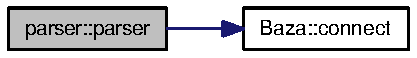
\includegraphics[width=118pt]{dd/dad/a00005_9f881c43df7d37da2d6dee1e89ee5f1f_cgraph}
\end{center}
\end{figure}


\subsection{Dokumentacja funkcji składowych}
\hypertarget{a00005_272ecc740702b4f48efdb8469b414b24}{
\index{parser@{parser}!czytanie\_\-z\_\-socketa@{czytanie\_\-z\_\-socketa}}
\index{czytanie\_\-z\_\-socketa@{czytanie\_\-z\_\-socketa}!parser@{parser}}
\subsubsection[{czytanie\_\-z\_\-socketa}]{\setlength{\rightskip}{0pt plus 5cm}std::string parser::czytanie\_\-z\_\-socketa ()\hspace{0.3cm}{\tt  \mbox{[}private\mbox{]}}}}
\label{dd/dad/a00005_272ecc740702b4f48efdb8469b414b24}


\hypertarget{a00005_96f941201d172eeaf2fb4d8429edfc0c}{
\index{parser@{parser}!lista\_\-plikow@{lista\_\-plikow}}
\index{lista\_\-plikow@{lista\_\-plikow}!parser@{parser}}
\subsubsection[{lista\_\-plikow}]{\setlength{\rightskip}{0pt plus 5cm}void parser::lista\_\-plikow (std::string {\em uzytkownik})\hspace{0.3cm}{\tt  \mbox{[}private\mbox{]}}}}
\label{dd/dad/a00005_96f941201d172eeaf2fb4d8429edfc0c}


Wysyła listę plików użytkownika 'uzytkownik'. 



Here is the caller graph for this function:\nopagebreak
\begin{figure}[H]
\begin{center}
\leavevmode
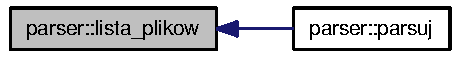
\includegraphics[width=128pt]{dd/dad/a00005_96f941201d172eeaf2fb4d8429edfc0c_icgraph}
\end{center}
\end{figure}
\hypertarget{a00005_71abf468eb72a833dbd6c8a895b66b52}{
\index{parser@{parser}!logowanie@{logowanie}}
\index{logowanie@{logowanie}!parser@{parser}}
\subsubsection[{logowanie}]{\setlength{\rightskip}{0pt plus 5cm}bool parser::logowanie (std::string {\em login}, \/  std::string {\em haslo})\hspace{0.3cm}{\tt  \mbox{[}private\mbox{]}}}}
\label{dd/dad/a00005_71abf468eb72a833dbd6c8a895b66b52}


Loguje klienta po przetworzeniu xmla odebranego od niego i sparsownaiu go w void \hyperlink{a00005_9ce7290217bd14e4efcbe2cad32ccf95}{parsuj()}. 



Here is the caller graph for this function:\nopagebreak
\begin{figure}[H]
\begin{center}
\leavevmode
\includegraphics[width=124pt]{dd/dad/a00005_71abf468eb72a833dbd6c8a895b66b52_icgraph}
\end{center}
\end{figure}
\hypertarget{a00005_4e084ae10e8498b171c44a0138597d2e}{
\index{parser@{parser}!odbieranie\_\-plikow@{odbieranie\_\-plikow}}
\index{odbieranie\_\-plikow@{odbieranie\_\-plikow}!parser@{parser}}
\subsubsection[{odbieranie\_\-plikow}]{\setlength{\rightskip}{0pt plus 5cm}void parser::odbieranie\_\-plikow (xmlpp::TextReader \& {\em reader}, \/  std::string {\em uzytkownik})\hspace{0.3cm}{\tt  \mbox{[}private\mbox{]}}}}
\label{dd/dad/a00005_4e084ae10e8498b171c44a0138597d2e}


Odbiera plik od użytkownika i umieszcza na serwerze. 



Here is the caller graph for this function:\nopagebreak
\begin{figure}[H]
\begin{center}
\leavevmode
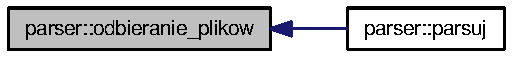
\includegraphics[width=141pt]{dd/dad/a00005_4e084ae10e8498b171c44a0138597d2e_icgraph}
\end{center}
\end{figure}
\hypertarget{a00005_e45404aec82f8c70a023bdc365c74287}{
\index{parser@{parser}!Odpowiedz@{Odpowiedz}}
\index{Odpowiedz@{Odpowiedz}!parser@{parser}}
\subsubsection[{Odpowiedz}]{\setlength{\rightskip}{0pt plus 5cm}void parser::Odpowiedz (int {\em nr\_\-odpowiedzi}, \/  int {\em nr\_\-operacji}, \/  std::string {\em odp})\hspace{0.3cm}{\tt  \mbox{[}private\mbox{]}}}}
\label{dd/dad/a00005_e45404aec82f8c70a023bdc365c74287}


Wysyła odpowiedź wielolinijkową zależnie od podanego i gdzie i jak w void \hyperlink{a00005_49d270636d2f3d5376c3cba62b5ea839}{Odpowiedz(int i, int numer\_\-operacji)};. 

\hypertarget{a00005_49d270636d2f3d5376c3cba62b5ea839}{
\index{parser@{parser}!Odpowiedz@{Odpowiedz}}
\index{Odpowiedz@{Odpowiedz}!parser@{parser}}
\subsubsection[{Odpowiedz}]{\setlength{\rightskip}{0pt plus 5cm}void parser::Odpowiedz (int {\em nr\_\-odpowiedzi}, \/  int {\em numer\_\-operacji} = {\tt -1})\hspace{0.3cm}{\tt  \mbox{[}private\mbox{]}}}}
\label{dd/dad/a00005_49d270636d2f3d5376c3cba62b5ea839}


Wysyła odpowiedź jednolinijkową zależnie od podanego i \begin{Desc}
\item[Parametry:]
\begin{description}
\item[{\em nr\_\-odpowiedzi}]Numer odpowiedzi 400 - bledne zapytanie 401 - bledny numer sesji 402 - podany plik istnieje (w przypadku wysylania pliku) 403 - wewnetrzny blad serwera 404 - podany plik nie istnieje 405 - błąd odbierania plikow 406 - wszystko OK \item[{\em numer\_\-operacji}]Numer operacji do której odnosi się podany nuemr odpowiedzi \end{description}
\end{Desc}


Here is the caller graph for this function:\nopagebreak
\begin{figure}[H]
\begin{center}
\leavevmode
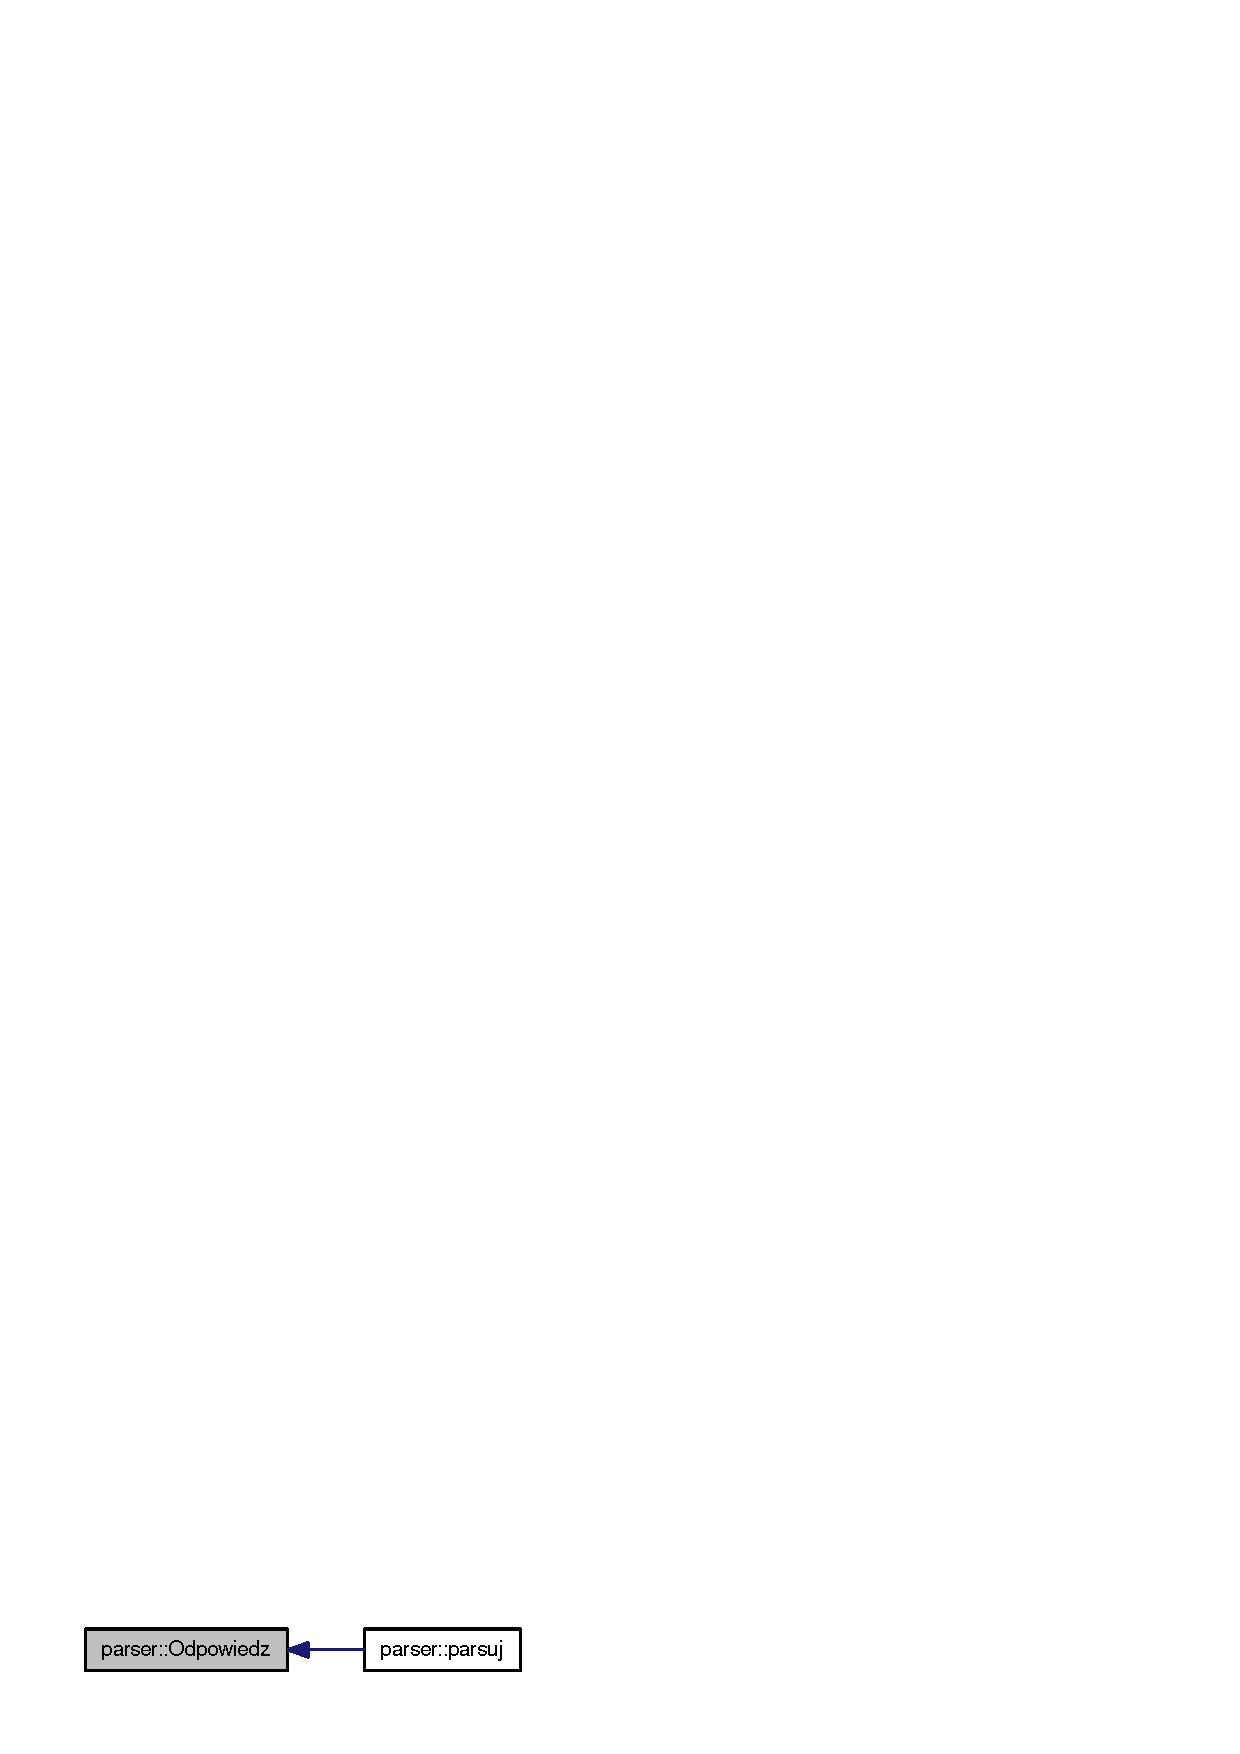
\includegraphics[width=127pt]{dd/dad/a00005_49d270636d2f3d5376c3cba62b5ea839_icgraph}
\end{center}
\end{figure}
\hypertarget{a00005_6a29174f787861caadc6c2e34b99f8c0}{
\index{parser@{parser}!odpowiedz\_\-login@{odpowiedz\_\-login}}
\index{odpowiedz\_\-login@{odpowiedz\_\-login}!parser@{parser}}
\subsubsection[{odpowiedz\_\-login}]{\setlength{\rightskip}{0pt plus 5cm}void parser::odpowiedz\_\-login (int {\em i})\hspace{0.3cm}{\tt  \mbox{[}private\mbox{]}}}}
\label{dd/dad/a00005_6a29174f787861caadc6c2e34b99f8c0}


Wysyła odpowiedź do logowania na podstawie podaneg i gdzie 0 - Logowanie przebieglo prawidlowo; 1 - błęde hasło lub login; 2 - nieoczekiwany błąd serwera; 3 - błędne zapytanie 

Here is the caller graph for this function:\nopagebreak
\begin{figure}[H]
\begin{center}
\leavevmode
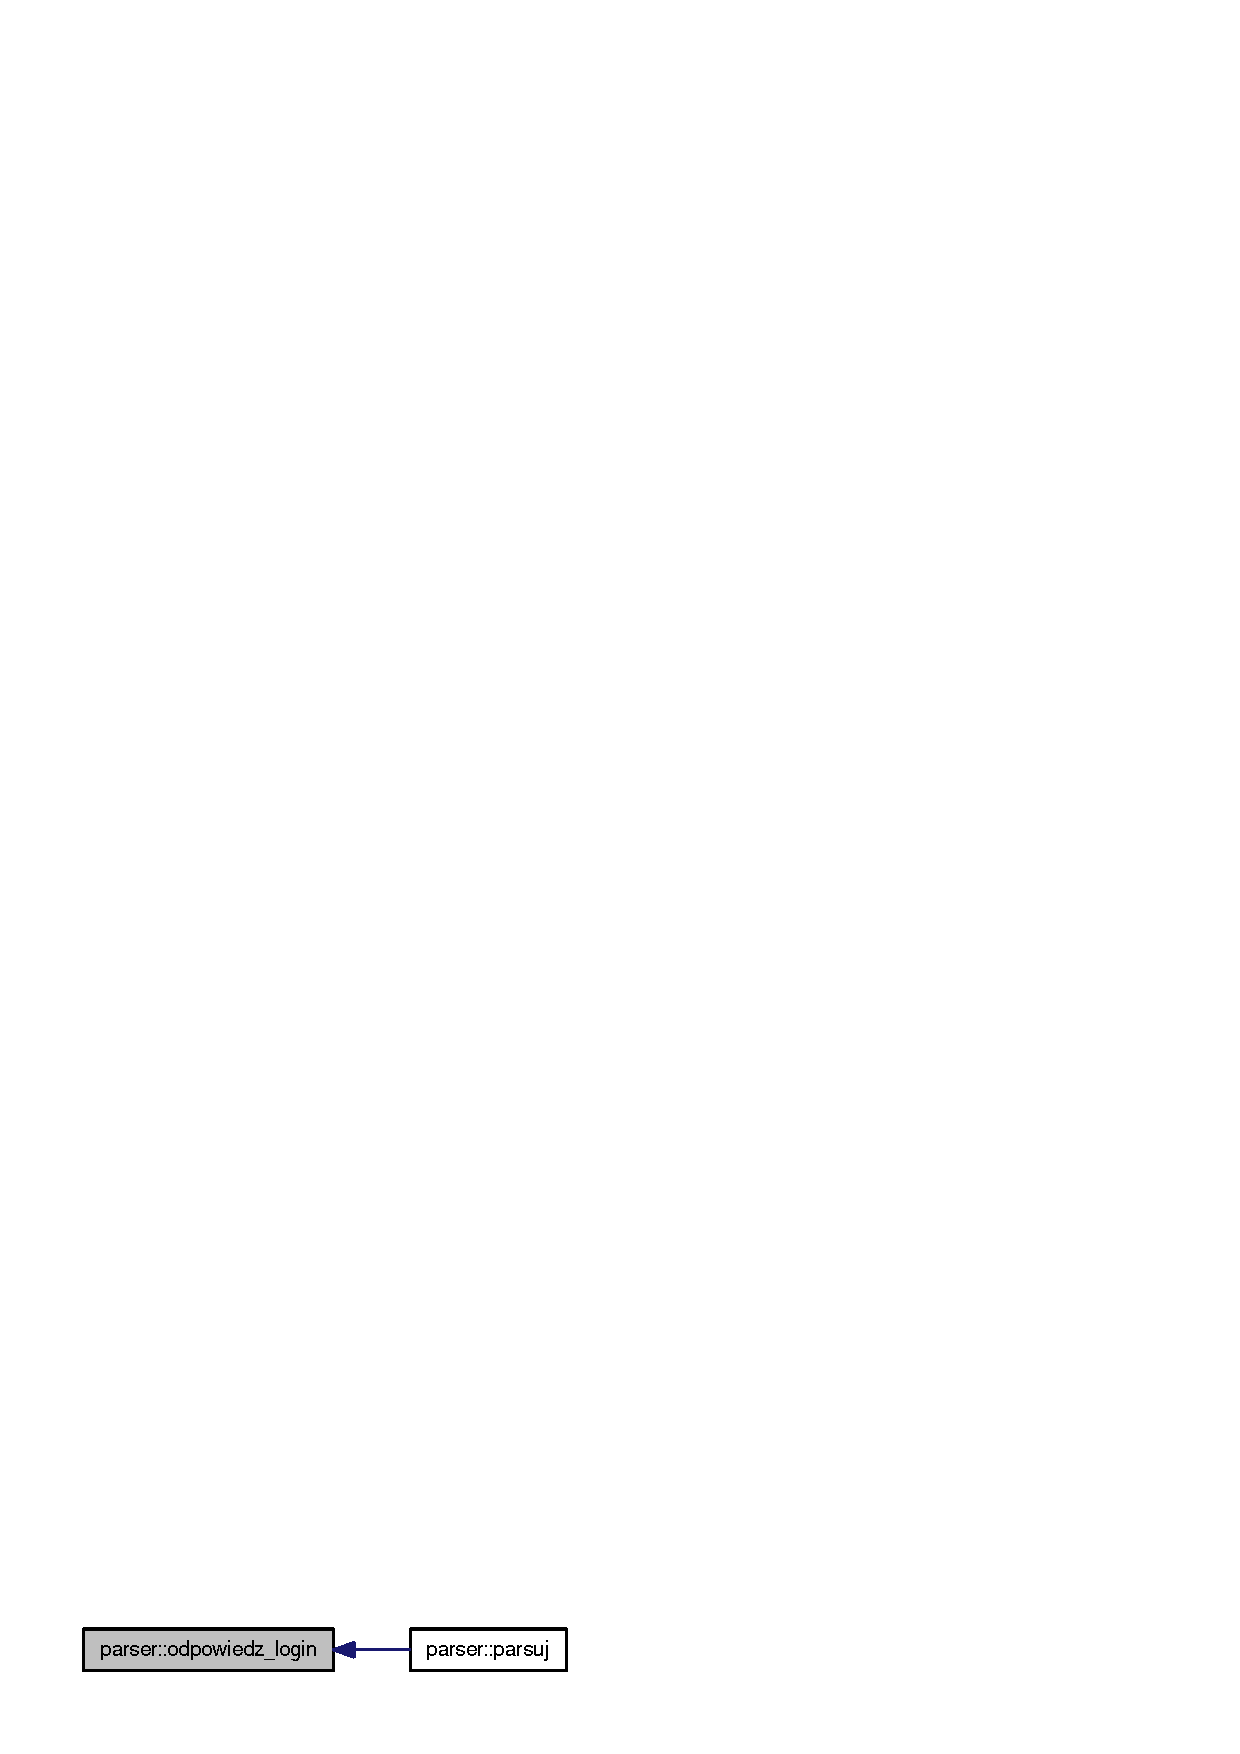
\includegraphics[width=138pt]{dd/dad/a00005_6a29174f787861caadc6c2e34b99f8c0_icgraph}
\end{center}
\end{figure}
\hypertarget{a00005_9ce7290217bd14e4efcbe2cad32ccf95}{
\index{parser@{parser}!parsuj@{parsuj}}
\index{parsuj@{parsuj}!parser@{parser}}
\subsubsection[{parsuj}]{\setlength{\rightskip}{0pt plus 5cm}bool parser::parsuj (std::string \& {\em do\_\-parsowania})\hspace{0.3cm}{\tt  \mbox{[}private\mbox{]}}}}
\label{dd/dad/a00005_9ce7290217bd14e4efcbe2cad32ccf95}


Parsuje dane pobrane od klienta. 



Logowanie - Trzeba pamiętać że \hyperlink{a00005}{parser} umieszcza dodatkowo spację na końcu sparsowanych stringów

Sprawdzanie ilosci atrybutów

Przesun sie do atrybutu \char`\"{}login\char`\"{}

Zapisz login

Gdy brak takiego atrybutu to konczymy rozmowe

Przesun sie do atrybutu \char`\"{}haslo\char`\"{}

Gdy brak takiego atrybutu to konczymy rozmowe

Sprawdzamy czy login i haslo pasują

Jeżeli tak to dajemy klientowi ID sesji

Jeżeli nie to informujemy go o tym i kończymy

Brak loginu i hasła

Jeżeli polecenie od klienta

Sprawdzanie ilosci atrybutów

Przesun sie do atrybutu \char`\"{}idsesji\char`\"{}

Sprawdzamy czy zgadza się id\_\-sesji

Sprawdzamy czy istnieje argument \char`\"{}operacja\char`\"{}

Błędne zapytanie

Niezgodne id\_\-sesji

Brak id\_\-sesji

Brak atrybutów

Funkcja wysyłająca dane przez SOCKET

Funkcja sprawdzająca czy dla podanego loginu hasło jest prawidłowe, jeżeli tak to generuje id\_\-sesji

Trzeba pamiętać że zmienna haslo tak naprawde zawiera haslo i na końcu spację.

Krotka odpowiedz gdzie i - kod odpowiedzi

Odpowiedź z dodatkowymi informacjami gdzie i - kod odpowiedzi

Funkcja wysyłająca odpowiedź po prośbie o zalogowanie

Funkcja wywoływana tylko raz, rozpoczyna pobieranie informacji z SOCKETA i przekazuje je parserowi

Jeżeli użytkownik to \char`\"{}.\char`\"{} to znaczy ze żądanie jest o liste plików użytkownika zalogowanego

Prośba o listę plików użytkownika uzytkownik 

Definicja w linii 16 pliku parser.cpp.

Oto graf wywołań dla tej funkcji:\nopagebreak
\begin{figure}[H]
\begin{center}
\leavevmode
\includegraphics[width=203pt]{dd/dad/a00005_9ce7290217bd14e4efcbe2cad32ccf95_cgraph}
\end{center}
\end{figure}
\hypertarget{a00005_05500b74ebdcc1578ead4c31fca73a5b}{
\index{parser@{parser}!pobieranie\_\-listy\_\-plikow@{pobieranie\_\-listy\_\-plikow}}
\index{pobieranie\_\-listy\_\-plikow@{pobieranie\_\-listy\_\-plikow}!parser@{parser}}
\subsubsection[{pobieranie\_\-listy\_\-plikow}]{\setlength{\rightskip}{0pt plus 5cm}std::vector$<$std::string$>$ parser::pobieranie\_\-listy\_\-plikow (xmlpp::TextReader \& {\em reader})\hspace{0.3cm}{\tt  \mbox{[}private\mbox{]}}}}
\label{dd/dad/a00005_05500b74ebdcc1578ead4c31fca73a5b}


Przygotowuje listę plikow do wysłania do klienta. 

\hypertarget{a00005_7793913f528921aa22c4b6cc259a0a14}{
\index{parser@{parser}!start@{start}}
\index{start@{start}!parser@{parser}}
\subsubsection[{start}]{\setlength{\rightskip}{0pt plus 5cm}void parser::start ()}}
\label{dd/dad/a00005_7793913f528921aa22c4b6cc259a0a14}




Here is the caller graph for this function:\nopagebreak
\begin{figure}[H]
\begin{center}
\leavevmode
\includegraphics[width=94pt]{dd/dad/a00005_7793913f528921aa22c4b6cc259a0a14_icgraph}
\end{center}
\end{figure}
\hypertarget{a00005_7ef79f818429f70b9cb35c0a33b59a10}{
\index{parser@{parser}!usun\_\-pliki@{usun\_\-pliki}}
\index{usun\_\-pliki@{usun\_\-pliki}!parser@{parser}}
\subsubsection[{usun\_\-pliki}]{\setlength{\rightskip}{0pt plus 5cm}void parser::usun\_\-pliki (xmlpp::TextReader \& {\em reader}, \/  std::string {\em uzytkownik})\hspace{0.3cm}{\tt  \mbox{[}private\mbox{]}}}}
\label{dd/dad/a00005_7ef79f818429f70b9cb35c0a33b59a10}


Usuwa plik z serwera (jeszcze nie zaimplementowane). 



Here is the caller graph for this function:\nopagebreak
\begin{figure}[H]
\begin{center}
\leavevmode
\includegraphics[width=125pt]{dd/dad/a00005_7ef79f818429f70b9cb35c0a33b59a10_icgraph}
\end{center}
\end{figure}
\hypertarget{a00005_2f6aceaa94a28fc699e4f824f7622b51}{
\index{parser@{parser}!wyslij@{wyslij}}
\index{wyslij@{wyslij}!parser@{parser}}
\subsubsection[{wyslij}]{\setlength{\rightskip}{0pt plus 5cm}void parser::wyslij (std::string {\em w})\hspace{0.3cm}{\tt  \mbox{[}private\mbox{]}}}}
\label{dd/dad/a00005_2f6aceaa94a28fc699e4f824f7622b51}


Wysyła dane podane w stringu w dodatkowo wysyłając znak końca linii. 



Here is the caller graph for this function:\nopagebreak
\begin{figure}[H]
\begin{center}
\leavevmode
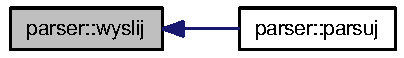
\includegraphics[width=115pt]{dd/dad/a00005_2f6aceaa94a28fc699e4f824f7622b51_icgraph}
\end{center}
\end{figure}
\hypertarget{a00005_e726284253cddec4b4b547a9d0254380}{
\index{parser@{parser}!wyslij\_\-plik@{wyslij\_\-plik}}
\index{wyslij\_\-plik@{wyslij\_\-plik}!parser@{parser}}
\subsubsection[{wyslij\_\-plik}]{\setlength{\rightskip}{0pt plus 5cm}void parser::wyslij\_\-plik (std::string {\em plik}, \/  std::string {\em uzytkownik}, \/  char {\em uprawnienia})\hspace{0.3cm}{\tt  \mbox{[}private\mbox{]}}}}
\label{dd/dad/a00005_e726284253cddec4b4b547a9d0254380}


wysyła plik podany w argumencie 

\hypertarget{a00005_0315a358465b40be344fddc7926c1316}{
\index{parser@{parser}!wysylanie\_\-plikow@{wysylanie\_\-plikow}}
\index{wysylanie\_\-plikow@{wysylanie\_\-plikow}!parser@{parser}}
\subsubsection[{wysylanie\_\-plikow}]{\setlength{\rightskip}{0pt plus 5cm}void parser::wysylanie\_\-plikow (xmlpp::TextReader \& {\em reader}, \/  std::string {\em uzytkownik}, \/  char {\em uprawnienia})\hspace{0.3cm}{\tt  \mbox{[}private\mbox{]}}}}
\label{dd/dad/a00005_0315a358465b40be344fddc7926c1316}


Odbiera od klienta informację jakie on chce pobrać pliki i przekazuje kazdy plik pojedynczo do \hyperlink{a00005_e726284253cddec4b4b547a9d0254380}{wyslij\_\-plik()}. 



Here is the caller graph for this function:\nopagebreak
\begin{figure}[H]
\begin{center}
\leavevmode
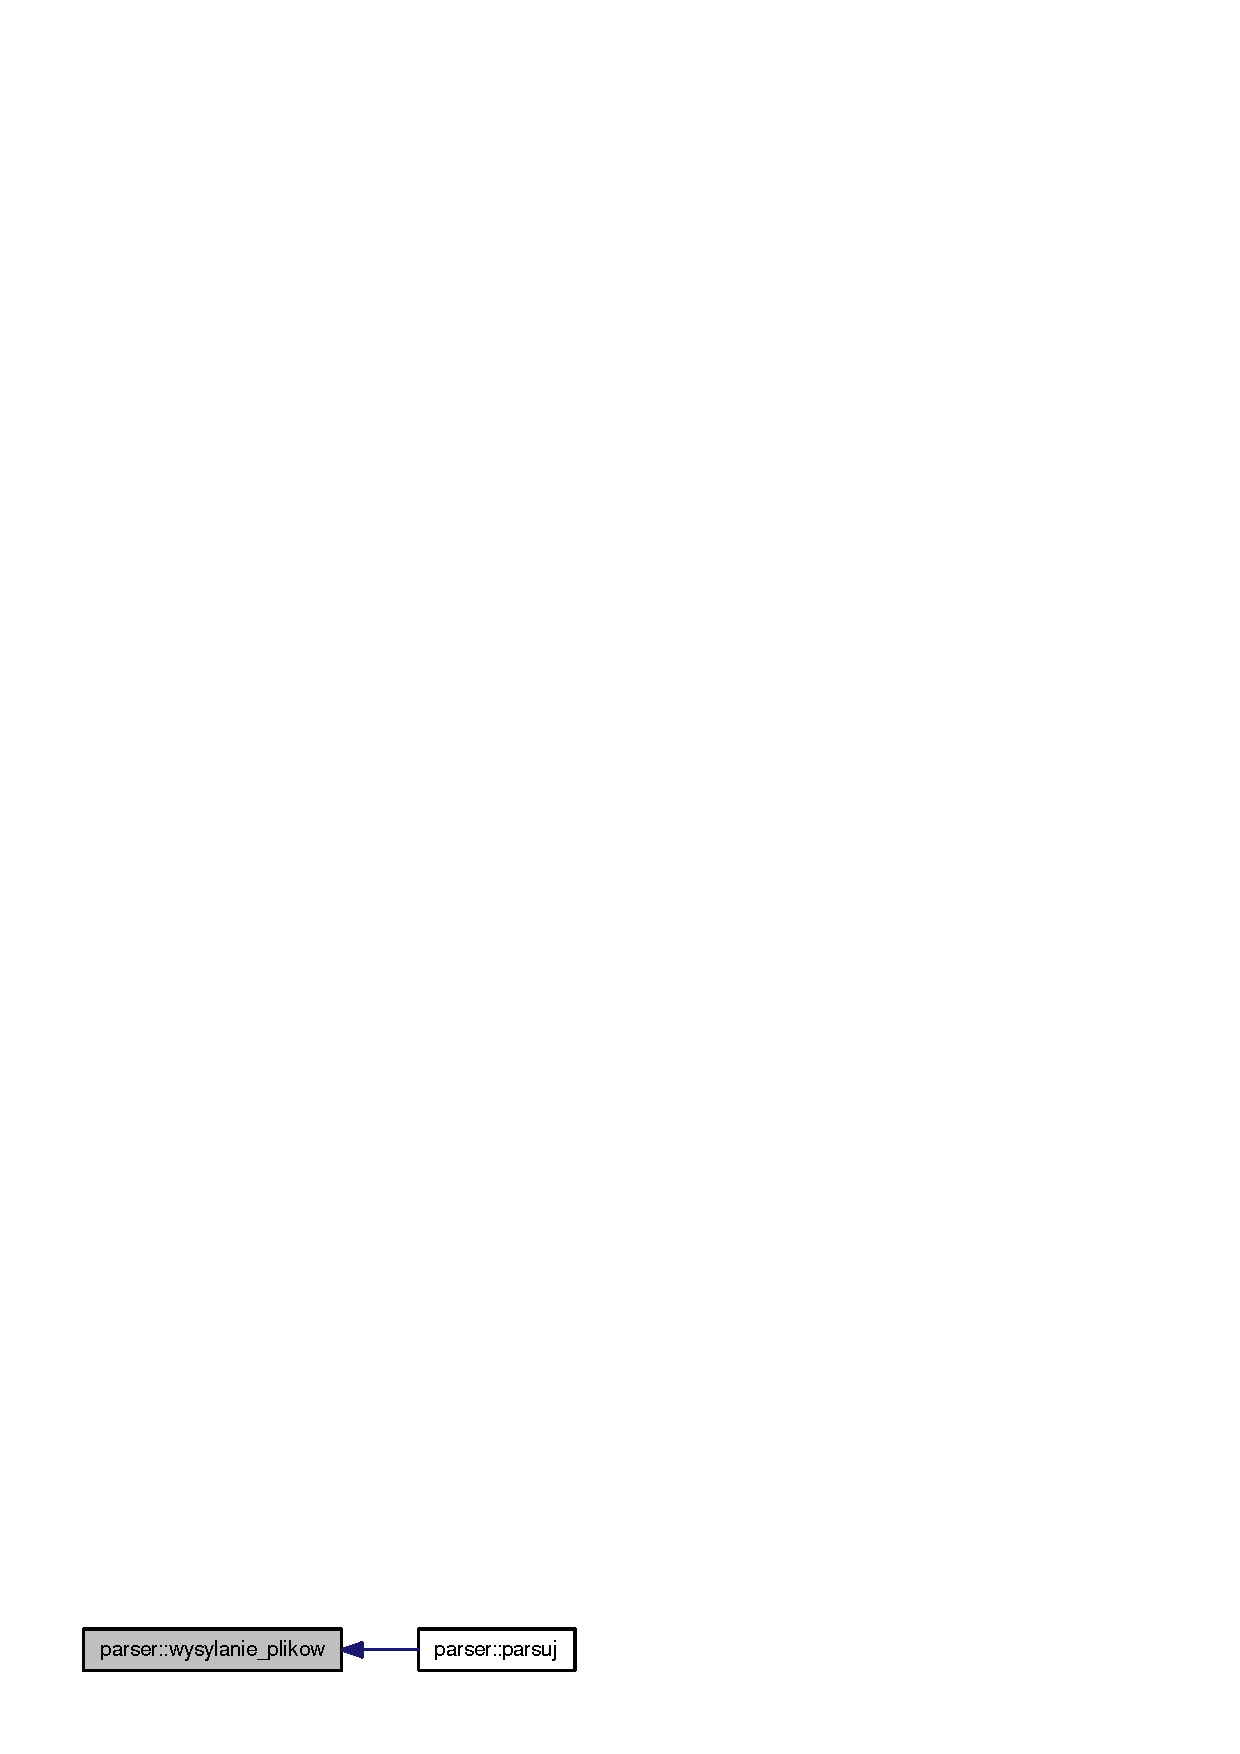
\includegraphics[width=140pt]{dd/dad/a00005_0315a358465b40be344fddc7926c1316_icgraph}
\end{center}
\end{figure}


\subsection{Dokumentacja atrybutów składowych}
\hypertarget{a00005_21b4b313249353e48f7ea67f534ee519}{
\index{parser@{parser}!baza@{baza}}
\index{baza@{baza}!parser@{parser}}
\subsubsection[{baza}]{\setlength{\rightskip}{0pt plus 5cm}{\bf Baza} {\bf parser::baza}\hspace{0.3cm}{\tt  \mbox{[}private\mbox{]}}}}
\label{dd/dad/a00005_21b4b313249353e48f7ea67f534ee519}


Clasa obsługująca bazę danych. 



Definicja w linii 45 pliku parser.hpp.\hypertarget{a00005_2e7575bebca6d0fd9f5a8bfe6fc652d0}{
\index{parser@{parser}!bufor@{bufor}}
\index{bufor@{bufor}!parser@{parser}}
\subsubsection[{bufor}]{\setlength{\rightskip}{0pt plus 5cm}char {\bf parser::bufor}\mbox{[}BUFSIZE\mbox{]}\hspace{0.3cm}{\tt  \mbox{[}private\mbox{]}}}}
\label{dd/dad/a00005_2e7575bebca6d0fd9f5a8bfe6fc652d0}


Bufor danych. 



Definicja w linii 43 pliku parser.hpp.\hypertarget{a00005_2fc04d16e2ba688c5b306a2ad6770039}{
\index{parser@{parser}!haslo@{haslo}}
\index{haslo@{haslo}!parser@{parser}}
\subsubsection[{haslo}]{\setlength{\rightskip}{0pt plus 5cm}std::string {\bf parser::haslo}\hspace{0.3cm}{\tt  \mbox{[}private\mbox{]}}}}
\label{dd/dad/a00005_2fc04d16e2ba688c5b306a2ad6770039}


Zmienna przechowująca haslo (w przyszlosci hash hasla) uzytkownika. 



Definicja w linii 37 pliku parser.hpp.\hypertarget{a00005_aa8407d10d299b524fa2f74532e537ac}{
\index{parser@{parser}!id\_\-sesji@{id\_\-sesji}}
\index{id\_\-sesji@{id\_\-sesji}!parser@{parser}}
\subsubsection[{id\_\-sesji}]{\setlength{\rightskip}{0pt plus 5cm}int {\bf parser::id\_\-sesji}\hspace{0.3cm}{\tt  \mbox{[}private\mbox{]}}}}
\label{dd/dad/a00005_aa8407d10d299b524fa2f74532e537ac}


Aktualny ID sesji potrzebny pryz kazdym polaczneiu. 



Definicja w linii 41 pliku parser.hpp.\hypertarget{a00005_8bb124a2f285074773d1b0ee62cf0cc0}{
\index{parser@{parser}!login@{login}}
\index{login@{login}!parser@{parser}}
\subsubsection[{login}]{\setlength{\rightskip}{0pt plus 5cm}std::string {\bf parser::login}\hspace{0.3cm}{\tt  \mbox{[}private\mbox{]}}}}
\label{dd/dad/a00005_8bb124a2f285074773d1b0ee62cf0cc0}


Zmienna przechowująca login uzytkownika. 



Definicja w linii 35 pliku parser.hpp.\hypertarget{a00005_835f5d6b548278a3e00d2c423336e903}{
\index{parser@{parser}!socket@{socket}}
\index{socket@{socket}!parser@{parser}}
\subsubsection[{socket}]{\setlength{\rightskip}{0pt plus 5cm}tcp::socket\& {\bf parser::socket}\hspace{0.3cm}{\tt  \mbox{[}private\mbox{]}}}}
\label{dd/dad/a00005_835f5d6b548278a3e00d2c423336e903}


socket uzywany do odbierania i wysyłania informacji 



Definicja w linii 33 pliku parser.hpp.

Dokumentacja dla tej klasy została wygenerowana z plików:\begin{CompactItemize}
\item 
\hyperlink{a00015}{parser.hpp}\item 
\hyperlink{a00014}{parser.cpp}\end{CompactItemize}
